\begin{pastexam}[label={px:ncku-106-ee-ds-06}]{成大電機所 106 學年度 簡答題第 2 題}
（簡答）

\textbf{(20 pts) Biconnected Components}

\begin{center}
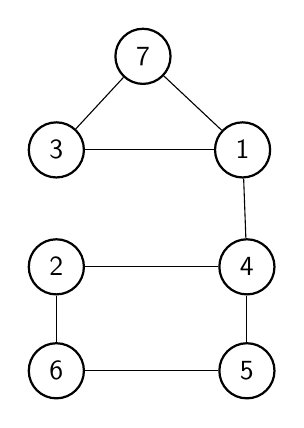
\begin{tikzpicture}[x=0.011cm,y=-0.011cm,v/.style={circle,draw,thick,inner sep=0pt,minimum size=7mm,font=\sffamily}]
\node[v] (n7) at (195,72) {7};
\node[v] (n3) at (95,180) {3};
\node[v] (n1) at (310,180) {1};
\node[v] (n2) at (95,315) {2};
\node[v] (n4) at (315,315) {4};
\node[v] (n6) at (95,435) {6};
\node[v] (n5) at (315,435) {5};
\draw (n7) -- (n3);
\draw (n7) -- (n1);
\draw (n3) -- (n1);
\draw (n1) -- (n4);
\draw (n2) -- (n4);
\draw (n2) -- (n6);
\draw (n4) -- (n5);
\draw (n6) -- (n5);
\end{tikzpicture}
\end{center}
\begin{enumerate}[label=\alph*.]
\item \textbf{(3 pts)} Show the depth-first search tree.
\item \textbf{(7 pts)} List the dfs numbers and low values of all nodes in a table.\\
(assume you start with node 1 and the search always start from a node with small number).
\item \textbf{(4 pts)} Show all articulation points and explain why they are the articulation points.
\item \textbf{(3 pts)} Give the definition of the back edge and show backward edges if the figure has.
\item \textbf{(3 pts)} Give the definition of the forward edge and show forward edges if the figure has.
\end{enumerate}
\end{pastexam}

\begin{pastsoln}
答案：a.\ 樹邊 $1\!-\!3$、$3\!-\!7$、$1\!-\!4$、$4\!-\!2$、$2\!-\!6$、$6\!-\!5$；b.\ 見下表；c.\ 割點是 $1$ 和 $4$；
d.\ 後向邊 $(7, 1)$、$(5, 4)$；e.\ 沒有前向邊。

圖的邊：$7\!-\!3$、$7\!-\!1$、$3\!-\!1$、$1\!-\!4$、$2\!-\!4$、$2\!-\!6$、$4\!-\!5$、$6\!-\!5$。 每個頂點的鄰居由小到大：
$1{:}\ 3, 4, 7$；$2{:}\ 4, 6$；$3{:}\ 1, 7$；$4{:}\ 1, 2, 5$；$5{:}\ 4, 6$；$6{:}\ 2, 5$；$7{:}\ 1, 3$。

\textbf{a.} 從 $1$ 出發，每次走編號最小的未拜訪鄰居（資結書第~21.4~節）：
\begin{itemize}
\item $1 \to 3$（$1$ 最小的鄰居）$\to 7$（$3$ 的鄰居 $1$ 已拜訪，走 $7$）。 $7$ 的鄰居 $1$、$3$ 都拜訪過，退回 $3$、
再退回 $1$。
\item $1 \to 4$（下一個鄰居）$\to 2$（$4$ 的鄰居 $1$ 已拜訪，走 $2$）$\to 6 \to 5$。 $5$ 的鄰居 $4$、$6$ 都拜訪過，
一路退回 $1$；$1$ 的最後一個鄰居 $7$ 已拜訪，結束。
\end{itemize}
DFS 樹（實線是樹邊，虛線是後向邊）：
\begin{center}
\begin{tikzpicture}[v/.style={circle,draw,thick,inner sep=0pt,minimum size=7mm,font=\sffamily},b/.style={densely dashed,->,>={Stealth[length=2mm]}}]
\node[v] (t1) at (0,0) {1};
\node[v] (t3) at (-1.6,-1.3) {3};
\node[v] (t7) at (-1.6,-2.6) {7};
\node[v] (t4) at (1.6,-1.3) {4};
\node[v] (t2) at (1.6,-2.6) {2};
\node[v] (t6) at (1.6,-3.9) {6};
\node[v] (t5) at (1.6,-5.2) {5};
\draw[thick] (t1)--(t3) (t3)--(t7) (t1)--(t4) (t4)--(t2) (t2)--(t6) (t6)--(t5);
\draw[b] (t7) to[bend left=40] (t1);
\draw[b] (t5) to[bend right=40] (t4);
\end{tikzpicture}
\end{center}

\textbf{b.} dfs number 是拜訪的先後（從 $1$ 開始），記作 $d$。
\[
\mathit{low}[u] = \min\bigl(d[u],\ \min\{\mathit{low}[w] : w \text{ 是 } u \text{ 的子節點}\},\
\min\{d[w] : (u, w) \text{ 是後向邊}\}\bigr)
\]
（資結書第~23.5~節）。 low 要等子節點都算完才確定，所以從後拜訪的往前算：
\begin{itemize}
\item $\mathit{low}[7] = \min(d[7], d[1]) = \min(3, 1) = 1$（後向邊 $7 \to 1$）；$\mathit{low}[3] = \min(2, \mathit{low}[7]) = 1$。
\item $\mathit{low}[5] = \min(7, d[4]) = 4$（後向邊 $5 \to 4$）；$\mathit{low}[6] = \min(6, 4) = 4$；
$\mathit{low}[2] = \min(5, 4) = 4$；$\mathit{low}[4] = \min(4, 4) = 4$。
\item $\mathit{low}[1] = \min(1, 1, 4) = 1$。
\end{itemize}
\begin{center}
\begin{tabular}{c*{7}{c}}
\toprule
頂點 & 1 & 2 & 3 & 4 & 5 & 6 & 7 \\
\midrule
$d$（dfs number） & 1 & 5 & 2 & 4 & 7 & 6 & 3 \\
$\mathit{low}$ & 1 & 4 & 1 & 4 & 4 & 4 & 1 \\
\bottomrule
\end{tabular}
\end{center}

\textbf{c.} 割點（articulation point）是拿掉之後圖會不連通的頂點。 判斷規則（資結書定理~23.8、23.9）：根是割點
若且唯若它在 DFS 樹裡至少有兩個子節點；非根的 $u$ 是割點若且唯若有某個子節點 $w$ 滿足
$\mathit{low}[w] \ge d[u]$。
\begin{itemize}
\item $1$（根）有兩個子節點 $3$、$4$，是割點。 理由：$3$ 的子樹 $\{3, 7\}$ 和 $4$ 的子樹 $\{4, 2, 6, 5\}$ 之間沒有
邊（無向圖的 DFS 沒有交叉邊），拿掉 $1$ 後兩塊就斷開。
\item $4$ 的子節點 $2$ 有 $\mathit{low}[2] = 4 \ge d[4] = 4$，是割點。 理由：$2$ 的子樹 $\{2, 6, 5\}$ 最高只能
回到 $4$，回不到 $4$ 的祖先 $1$；拿掉 $4$ 後 $\{2, 5, 6\}$ 和 $\{1, 3, 7\}$ 斷開。
\item 其他頂點都不是：$3$ 的子節點 $7$ 有 $\mathit{low}[7] = 1 < 2$；$2$ 的子節點 $6$ 有 $4 < 5$；$6$ 的子節點 $5$ 有
$4 < 6$；$5$、$7$ 是葉節點，沒有子節點。
\end{itemize}
割點是 $1$、$4$，雙連通元件是 $\{1, 3, 7\}$、$\{1, 4\}$、$\{2, 4, 5, 6\}$。

\textbf{d.} 後向邊（back edge）：DFS 時從 $u$ 看到一個已經拜訪、而且是 $u$ 的\textbf{祖先}（不是父節點）的頂點 $w$，
邊 $(u, w)$ 就是後向邊（資結書第~21.5~節）。 本圖的後向邊是 $(7, 1)$ 和 $(5, 4)$，就是圖上沒有被選成樹邊的那
兩條。 對無向圖做 DFS，每條邊不是樹邊就是後向邊（資結書定理~21.8），$8$ 條邊 $= 6$ 條樹邊 $+ 2$ 條後向邊。

\textbf{e.} 前向邊（forward edge）：DFS 時從 $u$ 看到一個已經拜訪完成、而且是 $u$ 的\textbf{子孫}（不是子節點）的
頂點 $w$，邊 $(u, w)$ 是前向邊。 這個分類用在有向圖。 本圖是無向圖，沒有前向邊：一條非樹邊 $\{u, w\}$ 一定是
先從比較晚拜訪的子孫那一端被看到（那時祖先還在進行中），所以被分類成後向邊。 例如 $\{1, 7\}$ 是在拜訪
$7$ 時就看到 $1$，記成後向邊 $(7, 1)$；等回到 $1$ 再看到 $7$ 時，這條邊已經分類過了。
\end{pastsoln}
